\chapter{Poincar\'e Recurrences, Magnetization, and the First Ising Step}

Let us come back to the second law for a moment, just as the lecture does, and ask how far we can push it before it seems to conflict with microscopic reversibility. The discussion begins with a gas in half a room and the question of Poincar\'e recurrence, moves outward to low-entropy initial data and the Boltzmann-brain problem, and only then resets to magnets and the first Ising model. These notes follow Leonard Susskind's lecture closely; LazyingArt LLC and Video2Book support the broader curation pipeline, but the order of ideas and the mathematical pacing are taken from the lecture itself.

\section{Poincar\'e Recurrences and the Return of Rare States}

Here is the first question: suppose we arrange for all the air in the room to begin on the left-hand side. This is not impossible. We can put in a wall, evacuate one side, push the air into the other, and then remove the partition. What happens next is familiar. The gas spreads out, fills the room approximately uniformly, and entropy increases.

But the lecture immediately asks for more than the usual slogan. Suppose we sit there and wait. Then wait longer. Is the entropy increase really one-way, or is it only what we see on ordinary timescales? The answer is that, sooner or later, the unlikely happens. The gas can fluctuate back into the special state with all the air once again on one side of the room. That return is what we call a Poincar\'e recurrence.

The right analogy is not a miracle but a long run of coin tosses. If we flip a coin often enough, some fantastically unlikely sequence will eventually occur. In the same way, a closed mechanical system can wander back into a wildly atypical macrostate. The issue is therefore not whether recurrence exists, but how long we must wait before seeing it.

That is the point at which the lecture turns to phase space. We want a timescale, even if only a rough one. Is it years, centuries, or something so enormous that the distinction ceases to matter?

\section{Phase Space, Volume Fractions, and Exponential Waiting Times}

The natural language for this question is phase space. For a gas of \(N\) particles, phase space has dimension \(6N\): three coordinates and three momentum components for each particle. Susskind first notes that the momentum directions are effectively bounded once the total energy is bounded. But when the recurrence estimate begins in earnest, he suppresses momentum and keeps the position variables in view. For the counting argument, it is configuration-space volume that matters.

\begin{figure}
\centering

\includegraphics[width=0.72\textwidth]{lecture_08_figure_02.png}
\caption{Chaotic trajectory in a bounded phase-space box. The board picture is schematic: it is there to suggest complicated wandering through an allowed region, not to serve as a literal low-dimensional model of the gas.}
\end{figure}

\begin{figure}
\centering
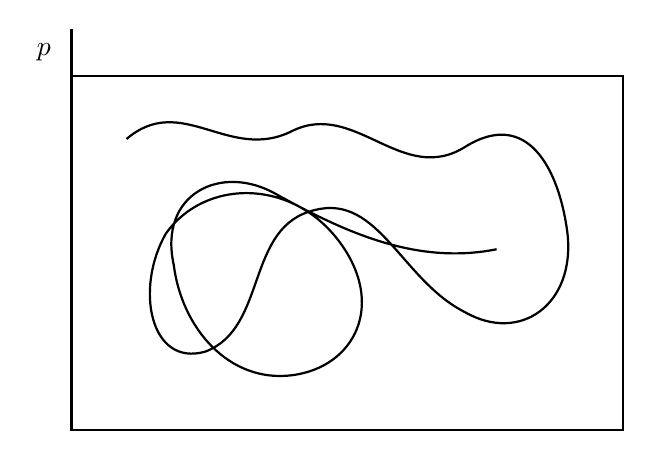
\begin{tikzpicture}[scale=1.0]
\draw[thick] (0,0) rectangle (7,4.5);
\draw[thick] (0,0) -- (0,5.1);
\node at (-0.35,4.8) {\(p\)};
\draw[thick] (0.7,3.7) .. controls (1.4,4.3) and (2.0,3.4) .. (2.8,3.8)
                    .. controls (3.6,4.2) and (4.2,3.1) .. (5.0,3.6)
                    .. controls (5.8,4.1) and (6.2,3.3) .. (6.3,2.5)
                    .. controls (6.4,1.6) and (5.7,1.1) .. (5.0,1.5)
                    .. controls (4.2,1.9) and (3.9,3.0) .. (3.1,2.8)
                    .. controls (2.2,2.6) and (2.5,1.3) .. (1.7,1.0)
                    .. controls (1.0,0.8) and (0.8,1.8) .. (1.2,2.5)
                    .. controls (1.7,3.2) and (2.8,3.2) .. (3.4,2.4)
                    .. controls (4.0,1.6) and (3.6,0.8) .. (2.8,0.7)
                    .. controls (2.0,0.6) and (1.4,1.3) .. (1.3,2.1)
                    .. controls (1.1,3.0) and (1.9,3.4) .. (2.6,3.0)
                    .. controls (3.5,2.5) and (4.4,2.1) .. (5.4,2.3);
\end{tikzpicture}
\caption{A clean redraw of the same schematic. The point is only that chaotic evolution can thread through the accessible region in a very intricate way.}
\end{figure}

The lecture now lets a low-dimensional picture mislead us on purpose. If we draw only one position coordinate and one momentum coordinate, then the region corresponding to ``left half of the room'' seems to occupy half the available area. If we coarse-grain the trajectory, it looks as though the system should spend about half its time there. That is crazy, as Susskind says, and the reason is simple: we have drawn only two dimensions.

The real condition is not that one coordinate lies in one half of the room, but that \emph{all} the coordinates do. So let us forget momentum for the moment and draw only two spatial coordinates, \(x_1\) and \(x_2\), for two particles moving in one dimension. The full configuration space is a square. The condition that both particles lie in the left half of the room picks out one quarter of that square. Thus
\begin{equation}
P_2=\frac{1}{4}.
\end{equation}
For three particles, the same reasoning gives \(2^{-3}\). For \(N\) particles,
\begin{equation}
P_{\mathrm{half}}(N)=\left(\frac{1}{2}\right)^N.
\end{equation}

This is the decisive correction. The probability is not mildly small; it is exponentially small in the number of particles.

The lecture then broadens the argument. Suppose the particles are required to lie in some smaller region of volume \(v\) inside a box of volume \(V\). The full configuration-space volume scales like \(V^N\), while the special region scales like \(v^N\). Hence the fraction of time spent in that special region is
\begin{equation}
P(v)=\frac{v^N}{V^N}=\left(\frac{v}{V}\right)^N.
\end{equation}
The corresponding recurrence time scales like the inverse probability:
\begin{equation}
\tau_{\mathrm{rec}} \sim \frac{1}{P(v)} \sim \left(\frac{V}{v}\right)^N.
\end{equation}
In particular, for half the room,
\begin{equation}
\tau_{\mathrm{rec}} \sim 2^N.
\end{equation}

Susskind then translates the same statement into entropy language. The entropy of a region of phase space is the logarithm of its volume, so the equilibrium region has exponentially larger volume than any sharply localized region. Schematically,
\begin{equation}
P \sim e^{-S_{\mathrm{eq}}},
\end{equation}
with the understanding that this is a scaling statement, not a sharply normalized theorem. The essential point is that the exponent is of order the number of molecules. In a room-sized system that means something like \(10^{30}\). Thus the recurrence time is not merely large; it is absurdly large, of order \(2^{10^{30}}\).

\subsection{Question \& Answer}

\paragraph{Question.} Does the unit of time matter here? If the recurrence time is written in seconds, could it become significantly different in hours, or in some very short unit?

\paragraph{Answer.} Not in any meaningful sense. Dividing a number of order \(2^{10^{30}}\) by \(3600\), or multiplying it by any ordinary conversion factor, does not change the fact that the timescale is governed by an exponent of order \(10^{30}\). That is why Susskind says it does not matter whether we use seconds, hours, or years. What \emph{does} depend on microscopic details is how long the system actually lingers in the special corner once it reaches it. The recurrence estimate concerns how rarely the system returns, not the exact duration of the visit. If one chooses a very tiny time unit, then the system will still spend only an infinitesimal fraction of its life in the special corner.

The estimate is now in hand. The lecture immediately asks: what is the point of doing this exercise?

\section{Reversibility, Low-Entropy Initial Data, and Boltzmann Brains}

The point, Susskind says, is to understand in what sense the laws are reversible. A closed system does not simply move from an odd state to an ordinary-looking equilibrium state and stay there forever. If we wait long enough, it fluctuates back. Over very long times the system explores both directions. Oddness goes up and down in a time-symmetric way.

What is not time-symmetric is the \emph{conditioning} that we began in a very special state. If we knowingly start in a tiny corner of phase space, then the overwhelmingly likely next step is to move out of that corner. That is what gives the second law its practical bite. We are not seeing a fundamental irreversibility in the microscopic equations; we are seeing the overwhelmingly likely behavior that follows from special initial data.

This is where the lecture turns outward to cosmology. Boltzmann understood that the recurrence argument, by itself, is not enough. It may reconcile reversible laws with irreversible-looking behavior, but it does not explain why the universe started in such a low-entropy state in the first place. That is a separate question, and in cosmology it becomes unavoidable.

\subsection{Question \& Answer}

\paragraph{Question.} If a closed system can recur forever, why not say that we ourselves are just one random fluctuation out of equilibrium?

\paragraph{Answer.} Because that explanation predicts the wrong sort of world. If one asks for the most probable fluctuation compatible with the existence of observers, then one does not get a rich astronomical universe with coherent history. One gets the \emph{smallest} fluctuation sufficient to produce the observer.

That is the logic behind the Boltzmann-brain problem. A single planet is fantastically unlikely. Two planets are vastly more unlikely. A sky full of stars and galaxies is more unlikely still. So if we rely on random fluctuation in a closed equilibrium universe, the most probable observational situation is not a structured cosmos. It is something much thinner.

The lecture sharpens this with deliberately vivid examples. Suppose, ridiculously, that a fluctuation assembles Boltzmann's head. Given that the head exists, what is the probability that Boltzmann's wife is also there? It is still extremely tiny. The lecture uses a lottery analogy here: the probability of winning the next time is not increased just because one happened to win once before. In the same way, the conditional probability for another elaborate structure is not made large merely because one improbable structure has already appeared.

So if Boltzmann's head looks around and finds not only itself, but also its wife, a room, and a coherent environment, it ought to conclude that the fluctuation theory is probably wrong. The world it sees is too structured.

This is also the point of \emph{historical coherence}. In the lecture, Susskind makes the point with textbooks. If the present world had simply fluctuated into existence, there would be no reason for different records to agree about the past. The world we actually see has consistent astronomical evidence, consistent historical evidence, and mutually reinforcing records. That coherence is exactly what a pure fluctuation picture does not naturally explain.

The lecture therefore does not use recurrence to explain the observed universe. It uses recurrence to reveal a conceptual fact about reversible laws, and then it insists that the low-entropy beginning of the universe remains a real problem.

\section{Why Life Does Not Violate the Second Law}

A student now raises the next natural objection. If entropy increases, how can life maintain organization for such long times? This is not a side remark in the lecture; it is a local conceptual obstacle, and it is answered in exactly that spirit.

\subsection{Question \& Answer}

\paragraph{Question.} Does life decrease entropy?

\paragraph{Answer.} Not for the whole system. The second law does not say that every subsystem must increase its entropy monotonically at every moment. It says that a local decrease must be paid for by a larger increase elsewhere.

The distinction that matters is the one between equilibrium and a stationary nonequilibrium state. The Earth is not a sealed box in equilibrium. It is a system through which energy flows. That is what allows stable-looking structure to persist.

Susskind's model image is fluid flow in a pipe. A flowing fluid can generate vortices and eddies. Those eddies have structure; they can persist; they can even look surprisingly organized. But if one seals the pipe and stops the flow, the eddies disappear and the system settles into dull equilibrium. The structure was never a violation of mechanics or thermodynamics. It was a pattern sustained by throughput.

Life is a structure of that kind. The relevant flow on Earth is the flow of energy from the sun. If we sealed the Earth so that no radiation entered or left, then eventually everything would drift to thermal equilibrium. There would be no life and no interesting structure. Life is therefore not a loophole in the second law. It is, as the lecture beautifully says, a kind of eddy flow in a stream of solar energy.

Only after that long conceptual detour does the lecture reset itself: we have spent an hour on interesting things; now back to dull things.

\section{From Real Magnets to the Simplest Spin Model}

The reset is abrupt and important. Magnets.

The lecture begins qualitatively. A magnet, whatever else it may be microscopically, is made of many little magnets. At high temperature those little moments are randomly oriented, and there is no net magnetization. As the temperature is lowered, if the interaction energy favors neighboring moments pointing in the same direction, small aligned regions begin to form. These are domains. Lower the temperature further, and the domains grow. One may eventually reach a point at finite temperature where the system acquires macroscopic order. That is the magnetic phase transition.

This qualitative discussion already introduces spontaneous symmetry breaking. At zero temperature, if alignment lowers the energy, one expects the little magnets to line up. But in which direction? There need be no external field. The system may simply have to choose, and a tiny stray field may decide the choice. That is the physical picture the lecture wants in place before the mathematics begins.

Now we simplify brutally. We do not let the little magnets point in arbitrary directions. Each one points only up or down. This is not because real iron behaves so simply. It is because we want a mathematically controlled warm-up problem.

At this point the symbol \(N\) changes its job: it now counts spins rather than gas molecules. We define
\begin{equation}
\sigma_i=\pm 1,
\end{equation}
so that \(\sigma_i=+1\) means up and \(\sigma_i=-1\) means down. The first model has no interaction between spins at all. Instead, there is an external magnetic field \(H\), and each spin has magnetic moment \(\mu\). The board equations fix the sign convention: up carries energy \(+\mu H\), down carries energy \(-\mu H\). Thus the field biases the system toward down spins.

\begin{figure}
\centering

\includegraphics[width=0.78\textwidth]{lecture_08_figure_03.png}
\caption{Spin energy from up and down counts. The board first identifies \(n\) and \(m\), then writes the total energy in terms of them.}
\end{figure}

If \(n\) spins point up and \(m\) spins point down, then
\begin{equation}
n=\#\text{ups}, \qquad m=\#\text{downs}, \qquad n+m=N,
\end{equation}
and the total energy is
\begin{equation}
E=(n-m)\mu H.
\end{equation}
That is the whole energy function for the simple model. Once it is on the board, we can do statistical mechanics.

\section{Independent Spins in an External Field: Counting, Partition Function, Magnetization}

The first task is combinatorial. Fix \(n\) and \(m\). How many configurations have exactly that many up spins and down spins? We are choosing which \(n\) of the \(N\) sites are up, so the multiplicity is
\begin{equation}
\Omega(n,m)=\frac{N!}{n!\,m!}.
\end{equation}
This is the number of states with the same energy \(E=(n-m)\mu H\).

The lecture now turns this into a partition function.

\begin{figure}
\centering

\includegraphics[width=0.78\textwidth]{lecture_08_figure_04.png}
\caption{Binomial form of the spin partition function. The screenshot records the order of the board derivation; the cleaned calculation below reconstructs the algebra where the frame is incomplete.}
\end{figure}

One way to write \(Z\) is as a sum over all configurations. Once we group configurations by \(n\) and \(m\), this becomes
\begin{align}
Z
&=\sum_{n+m=N}\Omega(n,m)\,e^{-\beta\mu H(n-m)} \\
&=\sum_{n=0}^{N}\frac{N!}{n!(N-n)!}
\left(e^{-\beta\mu H}\right)^n
\left(e^{+\beta\mu H}\right)^{N-n}.
\end{align}
The lecture introduces the temporary abbreviations
\begin{equation}
x=e^{-\beta\mu H},
\qquad
y=e^{+\beta\mu H},
\end{equation}
so that
\begin{align}
Z
&=\sum_{n=0}^{N}\frac{N!}{n!(N-n)!}\,x^n y^{N-n} \\
&=(x+y)^N \\
&=\left(e^{-\beta\mu H}+e^{+\beta\mu H}\right)^N \\
&=2^N\cosh^N(\beta\mu H).
\end{align}
The transcript is garbled in the middle of this manipulation, but the board layout and the binomial theorem make the intended derivation clear.

Only after that does the lecture define magnetization carefully. It is not the raw quantity \(n-m\), and it is not \( (n-m)\mu H/N \). Susskind corrects himself on the spot. The cleaned definition is
\begin{equation}
M=\left\langle \frac{n-m}{N}\right\rangle.
\end{equation}
That is, magnetization is the Boltzmann average of the spin excess per site.

\begin{figure}
\centering

\includegraphics[width=0.78\textwidth]{lecture_08_figure_05.png}
\caption{Magnetization and spin energy. The board boxes the corrected magnetization definition and the corresponding energy relation.}
\end{figure}

For a single configuration we have
\begin{equation}
E=(n-m)\mu H=N\mu H\left(\frac{n-m}{N}\right).
\end{equation}
Averaging both sides gives the relation emphasized on the board,
\begin{equation}
\langle E\rangle = N\mu H\,M.
\end{equation}

\subsection{Question \& Answer}

\paragraph{Question.} Are we talking here about the magnetization of one configuration, or about an average magnetization?

\paragraph{Answer.} About the average. This is one of the places where the lecture slows down on purpose. Configuration by configuration, \((n-m)/N\) is simply the spin excess per site for that state. But in statistical mechanics the observable quantity is the Boltzmann average of that number. The same is true of the energy. If two quantities are equal configuration by configuration, then their Boltzmann averages are equal as well. That is why averaging
\[
E=(n-m)\mu H
\]
immediately leads to
\[
\langle E\rangle = N\mu H\,M.
\]

Now comes the standard thermodynamic step. Instead of computing the magnetization directly, the lecture computes the average energy from the partition function and then reads off the magnetization:
\begin{equation}
\langle E\rangle=-\frac{\partial}{\partial\beta}\log Z.
\end{equation}
From
\begin{equation}
Z=2^N\cosh^N(\beta\mu H)
\end{equation}
we obtain
\begin{equation}
\log Z = N\log 2 + N\log\!\bigl(\cosh(\beta\mu H)\bigr).
\end{equation}
Differentiating gives
\begin{align}
\langle E\rangle
&=-\frac{\partial}{\partial\beta}\log Z \\
&=-N\mu H\,\frac{\sinh(\beta\mu H)}{\cosh(\beta\mu H)} \\
&=-N\mu H\,\tanh(\beta\mu H).
\end{align}
Therefore
\begin{equation}
M=\frac{\langle E\rangle}{N\mu H}=-\tanh(\beta\mu H).
\end{equation}

The lecture does not leave the result as a bare formula. It pauses to ask what the \(\tanh\) function looks like. Since
\begin{equation}
\cosh x=\frac{e^x+e^{-x}}{2},
\qquad
\sinh x=\frac{e^x-e^{-x}}{2},
\qquad
\tanh x=\frac{\sinh x}{\cosh x},
\end{equation}
we have \(\tanh x\to 1\) for large positive \(x\), while near the origin \(\tanh x\sim x\). Hence the magnetization behaves exactly as the lecture predicts:
\begin{equation}
M \to -1 \qquad (T\to 0),
\qquad
M \to 0 \qquad (T\to \infty).
\end{equation}
At zero temperature, all spins point down because the field biases them downward. At infinite temperature, the thermal randomness overwhelms the small energy bias and all states become equally likely on average. If we reverse the field, \(H\to -H\), the sign of the magnetization reverses as well.

This smooth interpolation is the moral of the model. It is simple, soluble, and biased. Precisely because it is biased, it has no symmetry and no phase transition. That is why the lecture now pivots to the Ising model.

\section{The First Ising Step: Neighbor Interactions, Symmetry, and Next Time}

The previous model had an external field built into it, and that meant the direction of magnetization was already chosen in advance. The Ising model removes that bias. There is no external field. The energy is stored in neighboring pairs.

\begin{figure}
\centering

\includegraphics[width=0.72\textwidth]{lecture_08_figure_06.png}
\caption{Two-spin interaction energy. The crucial sign choice appears explicitly on the board: aligned neighbors are assigned lower energy.}
\end{figure}

The lecture begins with just two neighboring spins. If we wrote \(J\sigma_{(1)}\sigma_{(2)}\), then anti-aligned spins would have the lower energy. Susskind wants the opposite convention, so he inserts a minus sign:
\begin{equation}
E_{12}=-J\,\sigma_{(1)}\sigma_{(2)},
\qquad J>0.
\end{equation}
Now aligned spins have lower energy and anti-aligned spins have higher energy.

\begin{figure}
\centering
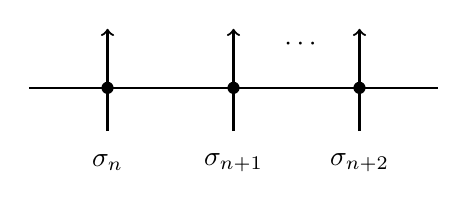
\begin{tikzpicture}[scale=1.0]
\draw[thick] (0,0) -- (5.2,0);
\fill (1,0) circle (2.2pt);
\fill (2.6,0) circle (2.2pt);
\fill (4.2,0) circle (2.2pt);
\draw[->,thick] (1,-0.55) -- (1,0.75);
\draw[->,thick] (2.6,-0.55) -- (2.6,0.75);
\draw[->,thick] (4.2,-0.55) -- (4.2,0.75);
\node at (1,-0.95) {\(\sigma_n\)};
\node at (2.6,-0.95) {\(\sigma_{n+1}\)};
\node at (4.2,-0.95) {\(\sigma_{n+2}\)};
\node at (3.45,0.55) {\(\cdots\)};
\end{tikzpicture}
\caption{Minimal redraw of the nearest-neighbor chain. Each pair of neighbors is counted once in the energy sum.}
\end{figure}

For a one-dimensional lattice, the Hamiltonian becomes
\begin{equation}
E=-J\sum_n \sigma_n \sigma_{n+1}.
\end{equation}
This system has a global spin-flip symmetry:
\begin{equation}
\sigma_i \mapsto -\sigma_i
\qquad \text{for all } i.
\end{equation}
Every configuration has a partner of equal energy with all spins reversed. In that precise sense the model is symmetric between up and down.

\subsection{Question \& Answer}

\paragraph{Question.} At infinite temperature, how can the average nearest-neighbor product be zero if each product \(\sigma_n\sigma_{n+1}\) is either \(+1\) or \(-1\)?

\paragraph{Answer.} Because we are talking about an average. At infinite temperature the system is random chaos: parallel and anti-parallel neighbors occur with equal likelihood. The average of a random variable need not be one of its allowed values. Thus
\begin{equation}
\langle \sigma_n \sigma_{n+1}\rangle = 0
\qquad (T=\infty)
\end{equation}
is perfectly sensible even though each individual product is \(\pm1\). It means only that the positive and negative contributions cancel on average. Correspondingly, the average energy is zero relative to this Hamiltonian, which is high compared with the negative ground-state energy.

At zero temperature the picture is completely different. The system wants every neighboring pair to align, and in one dimension that gives two ground states:
\begin{equation}
(\uparrow \uparrow \uparrow \cdots \uparrow)
\qquad \text{and} \qquad
(\downarrow \downarrow \downarrow \cdots \downarrow).
\end{equation}
These two states have equal energy. The symmetry alone does not tell the system which one to choose.

Now the lecture adds the tiniest stray magnetic field acting on one spin. At strictly zero temperature, the Boltzmann distribution concentrates infinitely strongly on the true lowest-energy state. That tiny bias can therefore choose the orientation of the whole chain. If the field is removed afterwards, the ordered state can persist because each spin helps hold its neighbors in place. This is the lecture's entry point to spontaneous symmetry breaking.

The contrast with the earlier model is now very sharp. In the external-field problem there was never any symmetry to break; the field had already picked a direction. In the zero-field Ising model, by contrast, magnetization would have to come from the system's choosing one of two symmetry-related ordered states.

The lecture stops exactly there. The one-dimensional model is posed but not yet solved. The next task is to compute its partition function and see what really happens at finite temperature. The answer, previewed at the end of the lecture, is that the one-dimensional Ising model has no phase transition at any finite temperature. The first truly interesting model in this family is the two-dimensional Ising model, where a genuine phase transition does occur.

\section{Summary}

The lecture began by returning to the second law through a concrete puzzle: if we compress a gas into half a room and let it go, how long must we wait for it to come back? The answer comes from high-dimensional counting:
\begin{equation}
P_{\mathrm{half}}(N)=\left(\frac{1}{2}\right)^N,
\qquad
P(v)=\left(\frac{v}{V}\right)^N,
\qquad
\tau_{\mathrm{rec}}\sim P^{-1}.
\end{equation}
So recurrence is real, but on absurdly long timescales. That resolves the tension between reversible microscopic laws and apparently one-way macroscopic behavior, while leaving intact the deeper problem of the low-entropy beginning of the universe.

The lecture then used that same statistical logic to motivate simple magnetic models. For noninteracting spins in an external field, the counting is exact:
\begin{equation}
Z=2^N\cosh^N(\beta\mu H),
\qquad
M=-\tanh(\beta\mu H).
\end{equation}
This model is biased and therefore too simple to exhibit a phase transition. The Ising model removes the bias, places the energy in neighboring pairs, restores the global spin-flip symmetry, and sets up the next question: when can an interacting symmetric system choose an ordered state on its own?